\chapter{Consistency and Evaluation}
\label{ch:consistency}

\begin{objectives}
\begin{itemize}
  \item Test whether a filter's covariance tells the truth, with NEES, NIS and $3\sigma$ coverage.
  \item Compute exact statistical bounds for single-run and Monte Carlo tests.
  \item Diagnose over- and under-confidence and tune noise parameters without cheating.
  \item Measure trajectory accuracy with ATE and RPE, using the alignment appropriate for VIO.
\end{itemize}
\end{objectives}

A filter produces two things: an estimate and a covariance. Most evaluations look only at the first. But a
filter with good average accuracy and a covariance that is too small is dangerous: it rejects valid measurements,
it reports false confidence to whatever consumes its output, and it eventually diverges. This chapter is about
checking the second output.

% ------------------------------------------------------------------------------
\section{What consistency means}

Recall from \cref{ch:prob} that a filter reporting $(\hat x_k, P_k)$ is consistent if its error $e_k = x_k\bminus\hat x_k$ has
zero mean and covariance $P_k$. Together with \cref{prop:innovation}, a consistent, correctly modeled filter
satisfies three testable properties:
\begin{enumerate}
  \item estimation errors are compatible with $P_k$ (tested with NEES, needs ground truth);
  \item innovations are compatible with $S_k$ (tested with NIS, needs no ground truth);
  \item innovations are white (tested with autocorrelation, needs no ground truth).
\end{enumerate}
The error must be computed with the manifold difference $\bminus$, using exactly the same convention as the
filter's covariance. Comparing a local-perturbation covariance with a global attitude error, or with an Euler
angle difference, produces meaningless statistics.

% ------------------------------------------------------------------------------
\section{Normalized estimation error squared}

\begin{definition}[NEES]
The normalized estimation error squared at time $k$ is
\begin{equation}
  \epsilon_k = e_k\T P_k\inv e_k, \qquad e_k = x_k\bminus\hat x_k .
\end{equation}
\end{definition}

If the filter is consistent and its errors are Gaussian, $\epsilon_k \sim \chi^2_n$ with $n = \dim e$ by
\cref{thm:mahalanobis-chi2}: its expected value is $n$. A single run gives one sample per time step, which is noisy.
Monte Carlo runs average it out. With $N$ independent runs, the average NEES
$\bar\epsilon_k = \frac1N\sum_{j=1}^N\epsilon_k^{(j)}$ satisfies $N\bar\epsilon_k \sim \chi^2_{Nn}$, so the two-sided 95\% interval is
\begin{equation}
  \left[\ \frac{\chi^2_{0.025}(Nn)}{N},\ \frac{\chi^2_{0.975}(Nn)}{N}\ \right].
  \label{eq:anees-bounds}
\end{equation}
For the 15-state IMU filter with $N = 50$ runs this is $[13.52, 16.56]$; for $N = 100$, $[13.95, 16.09]$.
\Cref{app:tables} lists more. Average NEES above the interval means overconfidence (errors larger than claimed);
below means underconfidence.

\begin{figure}[t]
  \centering
  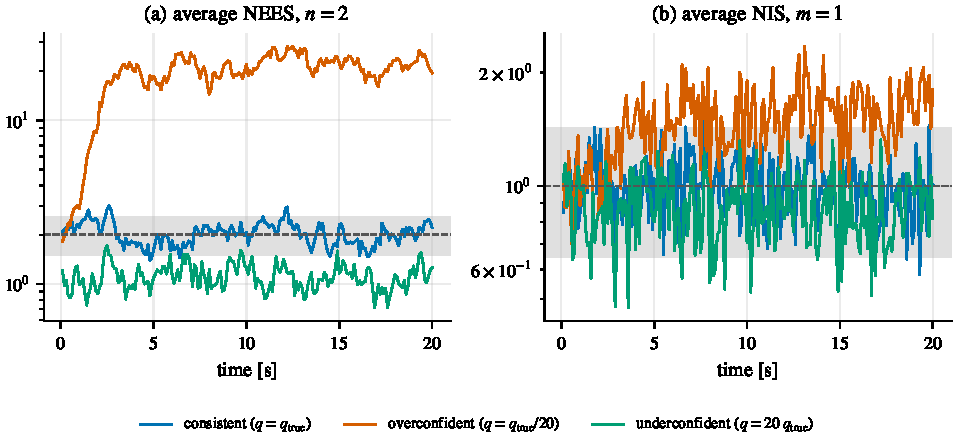
\includegraphics[width=\textwidth]{fig_nees.pdf}
  \caption{Consistency statistics of a constant-velocity filter over 50 Monte Carlo runs, with the 95\%
  acceptance region (gray) of \eqref{eq:anees-bounds}. Underestimating the process noise by a factor of 20 makes the
  filter overconfident: the NEES leaves the region by an order of magnitude, and the NIS rises above it. Overestimating
  it makes the filter underconfident: the NEES falls below the region. Note that the NIS of the underconfident filter
  is less clearly abnormal: NIS alone is a weak detector of underconfidence.}
  \label{fig:nees}
\end{figure}

\paragraph{Block NEES.} The NEES of the full state mixes well-estimated and poorly estimated blocks. Computing it
separately for position, velocity, attitude and biases, each with its own $3\times3$ block of $P$ and $\chi^2_3$ bounds, points
directly at the misbehaving part.

% ------------------------------------------------------------------------------
\section{Normalized innovation squared}

\begin{definition}[NIS]
$\nu_k = r_k\T S_k\inv r_k$, the same quantity the gate computes.
\end{definition}

Under consistency $\nu_k \sim \chi^2_m$ with $m = \dim r_k$. NIS needs no ground truth, so it is the main consistency
monitor on real data. Two summaries are useful: the fraction of updates with $\nu_k$ below its 95\% quantile, which
should be close to 95\% (Milestone 7), and the time-average of $\nu_k$, which should be close to $m$. If measurements have
different dimensions, normalize by $m_k$ or compare each against its own quantile.

\paragraph{$3\sigma$ coverage.} For each scalar component $i$, a consistent Gaussian error lies within $\pm3\sqrt{P_{ii}}$
99.7\% of the time. Plotting errors against their $3\sigma$ envelopes is the most readable diagnostic, and the coverage
fraction is a simple scalar summary. On EuRoC, Milestone 7 requires at least 95\% coverage for velocity and biases.
These states are not measured by the pose sensor, so their consistency is not circular.

% ------------------------------------------------------------------------------
\section{Diagnosing inconsistency}

\begin{table}[t]
\centering\small
\begin{tabularx}{\textwidth}{@{}l l X@{}}
\toprule
\textbf{NEES} & \textbf{NIS} & \textbf{Likely causes} \\
\midrule
high & high & process noise too small; wrong noise units (missing $\Dt$ or $\sqrt{\Dt}$); unmodeled IMU errors; integration error \\
high & normal & errors in directions the measurement does not see (unobservable states, e.g.\ yaw in VIO); wrong $\bminus$ convention in the evaluation \\
normal & high & measurement noise too small; outliers passing the gate; wrong $H$ \\
low & low & process or measurement noise too large \\
high, growing & normal & spurious information along unobservable directions (EKF inconsistency, \cref{ch:observability}) \\
spikes & spikes & time-synchronization errors; wrong extrinsics; bad initialization \\
\bottomrule
\end{tabularx}
\caption{Reading consistency statistics. Combinations narrow the search for the bug.}
\label{tab:consistency-diagnosis}
\end{table}

\Cref{tab:consistency-diagnosis} is a starting point for debugging. Two additional checks are valuable. First, plot each
residual component over time: a non-zero mean reveals a bias (wrong extrinsics, a wrong sign in $h$); slow oscillation
reveals correlated errors (a coloured noise the filter assumes white). Second, compare the covariance with Monte
Carlo statistics on synthetic data, where the truth is known exactly and the noise is exactly as modeled. If the filter
is inconsistent on synthetic data, the bug is in the filter. If it is consistent there but not on real data, the problem is
the model.

\subsection{Tuning without cheating}

\begin{enumerate}
  \item \textbf{Synthetic first.} With synthetic data generated with exactly the filter's noise parameters, there is
        nothing to tune: a consistent implementation must pass. Any failure is a bug.
  \item \textbf{Physically meaningful knobs only.} On real data, adjust the IMU noise densities (start from
        \cref{tab:euroc-imu}, inflate modestly for unmodeled effects) and the measurement noise (start from the pixel
        noise of the detector). Do not add arbitrary noise to arbitrary states.
  \item \textbf{Judge on consistency, not accuracy.} Choose parameters that make NIS and coverage statistics correct.
        Lower trajectory error obtained by making the filter inconsistent will not generalize.
  \item \textbf{Separate tuning from evaluation.} Tune on some sequences and report results on others.
  \item \textbf{Ground truth never enters the filter} except where explicitly allowed and logged (initialization).
\end{enumerate}

% ------------------------------------------------------------------------------
\section{Trajectory accuracy}

Consistency says whether the covariance is honest; accuracy says how small the errors are. VIO accuracy is
reported with two metrics~\cite{sturm2012tum, zhang2018tutorial}.

\subsection{Absolute trajectory error}

The estimated trajectory lives in a world frame that is only defined up to the unobservable directions, so it must
be aligned with the ground truth before comparing. Given time-associated positions $p_i$ (ground truth) and
$\hat p_i$ (estimate), find the transformation that best maps the estimate onto the truth, then compute
\begin{equation}
  \mathrm{ATE}_{\mathrm{RMSE}} = \Big(\frac1N\sum_{i=1}^N\big\|p_i - (R^\star\hat p_i + t^\star)\big\|^2\Big)^{1/2}.
\end{equation}
For rigid alignment, the optimal transformation has a closed form (Kabsch/Umeyama~\cite{umeyama1991}).

\begin{proposition}[Optimal rigid alignment]
\label{prop:umeyama}\label{sec:umeyama}
\index{Umeyama alignment}
Let $\mu$ and $\hat\mu$ be the means of the two point sets, $a_i = p_i - \mu$ and $b_i = \hat p_i - \hat\mu$ the centered points, and
$\Sigma_{ab} = \frac1N\sum_ia_ib_i\T = UDV\T$ an SVD. The minimizer of $\sum_i\|p_i - (R\hat p_i + t)\|^2$ over rotations $R$ and translations $t$ is
\begin{equation}
  R^\star = U\diag\big(1, 1, \det(UV\T)\big)V\T, \qquad t^\star = \mu - R^\star\hat\mu .
\end{equation}
\end{proposition}
\begin{proof}
For fixed $R$, the cost is a quadratic in $t$ minimized where its gradient vanishes, $\sum_i(p_i - R\hat p_i - t) = 0$, i.e.\ $t = \mu - R\hat\mu$: the alignment maps
centroid onto centroid. Substituting, the cost becomes $\sum_i\|a_i - Rb_i\|^2 = \sum_i(\|a_i\|^2 + \|b_i\|^2) - 2\sum_ia_i\T Rb_i$, so we must maximize
$\sum_ia_i\T Rb_i = \tr\big(R\sum_ib_ia_i\T\big) = N\tr(R\,VDU\T) = N\tr(D\,Z)$ with $Z = U\T RV$. $Z$ is orthogonal, so its diagonal entries are at most one in
magnitude, and $\tr(DZ) = \sum_id_iZ_{ii} \le \sum_id_i$, with equality for $Z = I$, i.e.\ $R = UV\T$. If $\det(UV\T) = -1$ this is a reflection, not a rotation; the
best rotation then flips the axis with the smallest singular value, $Z = \diag(1, 1, -1)$, which gives the stated formula.
\end{proof}

If the scale is also free (a similarity transform, needed for monocular vision without an IMU), the optimal scale is
$s^\star = \tr(D\,\diag(1, 1, \det(UV\T)))\big/\frac1N\sum_i\|b_i\|^2$, applied as $s^\star R^\star\hat p_i + t^\star$ with $t^\star = \mu - s^\star R^\star\hat\mu$.

\begin{keyidea}[align only what is unobservable]
Which transformation to allow depends on the estimator. Monocular vision alone has a free scale, so it uses a
similarity transform (7 DOF). VIO has metric scale and observable roll and pitch: its unobservable directions are
exactly translation and yaw. The appropriate alignment is therefore 4-DOF (translation plus a rotation about
gravity)~\cite{zhang2018tutorial}. A full 6-DOF alignment would also remove roll and pitch errors that the
estimator was responsible for.
\end{keyidea}

The 4-DOF alignment follows the same proof with $R$ restricted to rotations $R_z(\psi)$ about the vertical. For centered points $a = (x, y, z)$ (truth)
and $b = (\hat x, \hat y, \hat z)$ (estimate), $a\T R_z(\psi)b = (x\hat x + y\hat y)\cos\psi + (y\hat x - x\hat y)\sin\psi + z\hat z$, whose sum over the points is maximized by
\begin{equation}
  \psi^\star = \atantwo\Big(\sum_i(y_i\hat x_i - x_i\hat y_i),\ \sum_i(x_i\hat x_i + y_i\hat y_i)\Big),
  \label{eq:4dof-yaw}
\end{equation}
again with $t^\star = \mu - R_z(\psi^\star)\hat\mu$.

Milestone 10b reports ATE after SE(3) alignment, as in most published benchmarks; reporting the 4-DOF result
alongside it is more faithful to what VIO can know.

\subsection{Relative pose error}

ATE is dominated by the largest drift and depends on trajectory length and shape. The relative pose error (RPE)
compares relative motions over a fixed distance or time $\Delta$:
\begin{equation}
  E_i = \big(T_{i}\inv T_{i+\Delta}\big)\inv\big(\hat T_i\inv\hat T_{i+\Delta}\big),
\end{equation}
and reports statistics of the translation and rotation parts of $E_i$, often as a percentage of distance traveled. It
needs no global alignment and measures local drift, which is what odometry is about. The \code{evo}
package~\cite{grupp2017evo} computes both metrics with all the alignment variants.

\begin{projectlink}[Milestone 7]
M7 logs $\hat x$, $\diag(P)$, ground truth, NIS and NEES to a preallocated buffer, flushes it outside the hot loop, and
plots $3\sigma$ envelopes and NEES/NIS against their $\chi^2$ bounds from a single script. Exit criteria: average NEES inside
the 95\% interval for 15 DOF over most of a $\geq50$-run synthetic Monte Carlo; NIS within its per-update bound for about
95\% of updates; at least 95\% $3\sigma$ coverage of velocity and biases on MH\_01; zero allocations while logging.
\end{projectlink}

\begin{takeaways}
\begin{itemize}
  \item A filter must be judged on the honesty of its covariance as well as its accuracy.
  \item NEES needs ground truth and tests $P$; NIS needs none and tests $S$. Both are $\chi^2$ under consistency.
  \item Monte Carlo averages have exact bounds $[\chi^2_{0.025}(Nn), \chi^2_{0.975}(Nn)]/N$.
  \item Overconfidence (NEES too high) is the dangerous failure; NIS alone detects underconfidence poorly.
  \item Tune physically meaningful parameters for consistency, on synthetic data first.
  \item Report ATE after an alignment matched to the unobservable directions, and RPE for local drift.
\end{itemize}
\end{takeaways}

\begin{exercises}
  \item Show that the single-run NEES of a consistent 15-state filter exceeds its 95\% quantile 5\% of the time. Why
        is the Monte Carlo average a much sharper test?
  \item Reproduce \cref{fig:nees}. Then make only the measurement noise wrong instead of the process noise and compare
        the signatures.
  \item Derive the closed-form 4-DOF alignment above by maximizing $\sum_i p_i\T R_z(\psi)\hat p_i$ over $\psi$.
  \item Explain why the NEES of yaw in a VIO run on real data tends to grow over time even when the NIS looks
        healthy. (Revisit after \cref{ch:observability}.)
  \item Compute the RPE over 10~m segments for a trajectory with a constant yaw drift of $1^\circ$ per minute flying at
        1~m/s. How does it compare with the ATE after a 10-minute flight?
\end{exercises}
% Solutions to the exercises of Chapter 19.
\begin{solutions}
  \item If the filter is consistent and its errors Gaussian, $\epsilon_k = e_k\T P_k\inv e_k \sim \chi^2_{15}$ (\cref{thm:mahalanobis-chi2}). The 95\% quantile $\chi^2_{0.95}(15) = 25.0$ is
        by definition the value exceeded with probability 5\%, so a single run exceeds it at 5\% of its time steps. A single sample is a weak test:
        its two-sided 95\% range is $[6.3, 27.5]$, a factor of more than four, and a filter whose covariance is too small by 30\% still produces values
        inside it most of the time. Averaging over $N$ independent runs shrinks the spread: $N\bar\epsilon \sim \chi^2_{15N}$ has relative standard deviation
        $\sqrt{2/(15N)}$, and for $N = 50$ the interval is $[13.5, 16.6]$, about $\pm10\%$. A 30\% error now moves the average far outside it.

  \item In a simulation of the same kind as \cref{fig:nees} ($q = r = 1$, 50 runs of 200 steps), the average NEES ($n = 2$) and NIS ($m = 1$) after the
        transient are:
        \begin{center}\small
        \begin{tabular}{@{}l c c@{}}
        \toprule
        filter & NEES (band $[1.48, 2.59]$) & NIS (band $[0.65, 1.43]$) \\
        \midrule
        consistent & 1.9 & 1.00 \\
        $Q/20$ & 20.0 & 1.5 \\
        $20\,Q$ & 1.1 & 0.87 \\
        $R/20$ & 21.7 & 17.5 \\
        $20\,R$ & 1.0 & 0.08 \\
        \bottomrule
        \end{tabular}
        \end{center}
        Both kinds of error make the filter over- or underconfident in the NEES, but the NIS separates them. A wrong measurement noise enters $S$
        directly, so the NIS is wildly off ($17.5$ and $0.08$). A wrong process noise affects $S$ only through $HP^-H\T$, which the measurement noise partly
        masks, so the NIS moves much less ($1.5$ and $0.87$, the latter inside the band). Rule of thumb: NIS problems point at $R$ (or at outliers and
        wrong measurement models), NEES problems with a healthy NIS point at $Q$ or at unobservable directions (\cref{tab:consistency-diagnosis}).

  \item With centered points $a_i = (x_i, y_i, z_i)$ (truth) and $b_i = (\hat x_i, \hat y_i, \hat z_i)$ (estimate),
        \[
          \sum_ia_i\T R_z(\psi)b_i = \cos\psi\underbrace{\sum_i(x_i\hat x_i + y_i\hat y_i)}_{A} + \sin\psi\underbrace{\sum_i(y_i\hat x_i - x_i\hat y_i)}_{B} + \sum_iz_i\hat z_i .
        \]
        As a function of $\psi$ this is $\sqrt{A^2 + B^2}\cos(\psi - \psi_0) + \text{const}$ with $(\cos\psi_0, \sin\psi_0) \propto (A, B)$, so it is maximized at
        $\psi^\star = \atantwo(B, A)$, which is \eqref{eq:4dof-yaw}. (Setting the derivative $-A\sin\psi + B\cos\psi$
        to zero gives $\tan\psi = B/A$, which has two solutions; the $\atantwo$ picks the maximum rather than the minimum.) The translation follows
        as before: $t^\star = \mu - R_z(\psi^\star)\hat\mu$, which maps centroid onto centroid.

  \item The standard EKF linearizes at estimates that change over time, which makes the global yaw appear observable in its linearized model
        (\cref{ch:observability}). The filter then extracts spurious yaw information from measurements that contain none: its yaw variance shrinks,
        or grows more slowly than the true yaw error, which in VIO drifts like a random walk because nothing measures it. The NEES of yaw,
        $e_\psi^2/\sigma_\psi^2$, therefore grows steadily. The NIS stays healthy because innovations depend only on observable quantities (relative motion,
        roll, pitch, scale): an error along an unobservable direction changes no predicted measurement, so it cannot show up in the residuals
        (\cref{tab:consistency-diagnosis}, ``high, growing / normal'').

  \item A yaw drift of $1^\circ$ per minute is $\omega_d = 2.9\times10^{-4}$~rad/s. A 10~m segment takes 10~s at 1~m/s, during which the heading drifts by
        $0.167^\circ$: that is the rotational RPE. The translational RPE is the lateral offset accumulated within the segment, about
        $\tfrac12\omega_dv\,\Delta t^2 = 1.5$~cm (a simulation gives $1.4$~cm), i.e.\ $0.15\%$ of the distance travelled, and it is the same for every segment of the
        flight. For a straight 10-minute flight, by contrast, the estimated path bends into an arc of radius $v/\omega_d = 3.4$~km: the final position error is
        $\tfrac12\omega_dvT^2 = 52$~m, the RMS error without alignment 23~m, and after the best rigid alignment still $3.9$~m. The ATE grows quadratically
        with the duration and depends on the trajectory and on the alignment; the RPE does not grow and measures the drift rate itself, which is why
        odometry is compared with RPE and full trajectories with ATE.
\end{solutions}

